% =====================================================================================================
% ICML submission.  Numbers: ONLY from paper/RESULTS_MASTER.md (section refs like [R8b.5] in comments).
% Rules: paper/WRITING_PROMPT.md.  Argument: paper/STORY.md.
%
% STYLE FILES: download the official ICML style kit for the target year (icml20XX.sty, icml20XX.bst,
% algorithm*.sty, fancyhdr) into this folder and set \icmlstyle below. Until then the file compiles with a
% plain two-column fallback so you can write and check layout.
% PAGE LIMIT (check the current CFP): 8 pages of main text; references, impact statement and appendix unlimited.
% DOUBLE-BLIND: no names, no GitHub links with usernames; use an anonymous repository for code.
% =====================================================================================================
\def\icmlstyle{icml2026}   % <- change to the official style name once the files are in this folder
\IfFileExists{\icmlstyle.sty}{%
  \documentclass{article}
  \IfFileExists{microtype.sty}{\usepackage{microtype}}{}\usepackage{graphicx}\usepackage{booktabs}\usepackage{hyperref}
  \usepackage{\icmlstyle}  % submission mode = anonymous; add [accepted] only for camera-ready
  \def\usingicml{1}
}{%
  \documentclass[10pt,twocolumn]{article}
  \usepackage[margin=0.75in]{geometry}\IfFileExists{microtype.sty}{\usepackage{microtype}}{}\usepackage{graphicx}\usepackage{booktabs}
  \usepackage{hyperref}\usepackage{natbib}
}
\usepackage{amsmath,amssymb}
\usepackage{xcolor}
\usepackage{longtable}
\newcommand{\todo}[1]{\textcolor{red}{[TODO: #1]}}
\newcommand{\SC}{SC@50}
\graphicspath{{../figures/thickets-or-tilts/}}

\begin{document}

\ifdefined\usingicml
  \twocolumn[
  \icmltitle{What Does Random Weight Search Buy?\\Votes, Prompts and First-Order Tilts in RandOpt}
  \begin{icmlauthorlist}\icmlauthor{Anonymous Authors}{anon}\end{icmlauthorlist}
  \icmlaffiliation{anon}{Anonymous Institution}
  \icmlcorrespondingauthor{Anonymous}{anon@example.com}
  \vskip 0.3in]
  \printAffiliationsAndNotice{}
\else
  \title{What Does Random Weight Search Buy?\\Votes, Prompts and First-Order Tilts in RandOpt}
  \author{Anonymous Authors}\date{}\maketitle
\fi

% -----------------------------------------------------------------------------------------------------
\begin{abstract}
% Every number must match RESULTS_MASTER. Keep all qualifiers ("matches or beats", "no difference").
Random-perturbation post-training (RandOpt) samples thousands of Gaussian weight perturbations of a pretrained model,
keeps the best on a small selection set and majority-votes them, reportedly rivalling PPO and GRPO. We ask what the
weight search buys. Running RandOpt at its own settings in four rows (GSM8K with two Qwen models and OLMo-2-1B; GQA
with Qwen2.5-VL-3B), we reproduce its published numbers and decompose its gain into a vote and a shift in answers
shared across questions. Where the selected models barely beat the base model, self-consistency over 50 samples of the
unperturbed model beats RandOpt. Where RandOpt leads, its own prompt costs the base model 11.3 and 31.6 points and the
selected perturbations recover part of that accuracy. Choosing among a few prompts on RandOpt's own selection
questions (600 generations versus its 1,000,000) and then sampling matches or beats RandOpt in all four rows when the
candidates include a format-fixing prompt, and in three of four with public evaluation templates alone. With the
chosen prompt held fixed, RandOpt's search adds nothing over sampling in any row, and its selected models are no better
than the base model on test: what selection finds is specific to the prompt it runs under. A first-order account,
computed from the base model's gradient and each perturbation's noise with no fitted coefficients, tracks how
perturbations shift answer preferences ($r = 0.787$--$0.938$ across five models in two families), localizes the effect
to middle language layers and explains why selection favours shared shifts; it fails for vision weights, large
$\sigma$ and chain-of-thought correctness. Confirmatory tests were specified in plan locks committed before their
runs; we release all locks, data and code.
\end{abstract}

% -----------------------------------------------------------------------------------------------------
\section{Introduction}\label{sec:intro}
Random-perturbation post-training \citep{gan2026thickets} is a striking result. RandOpt samples thousands of Gaussian
perturbations of a pretrained model's weights, keeps those that score best on a small selection set, and majority-votes
their answers; it reportedly rivals PPO and GRPO on reasoning and vision benchmarks. Its authors read this as evidence
that diverse task experts are dense around pretrained weights, a ``neural thicket''. The method reproduces, and the
original paper itself notes that part of its GSM8K gain is a change in answer format. What is not yet known is what
the weight search contributes beyond things that are much cheaper to obtain.

We ask two questions. \emph{What does the weight search buy?} And \emph{what do the selected perturbations change in
the model's answers?} We answer the first with same-run comparisons at RandOpt's own settings, in four rows spanning
two tasks and two model families, against self-consistency at the same test-time budget, plus controls that each
isolate one component. We answer the second with a first-order account of how a perturbation shifts answer
preferences, which we test directly and whose limits we map.

The answer is short (Figures~\ref{fig:overview} and~\ref{fig:headline}). RandOpt's gain has two parts: a vote, and a
shift in the model's answers shared across questions. Where the selected models barely beat the base model, sampling
the unperturbed model votes better, and self-consistency beats RandOpt. Where RandOpt beats self-consistency, its own
prompt damages the base model (by 11.3 and 31.6 points) and the selected perturbations recover part of that accuracy.
Choosing among a few prompts on RandOpt's own 200 selection questions, at 0.06\% of its selection compute, then
sampling, matches or beats RandOpt in all four rows when the candidates include a format-fixing prompt, and in three
of four with public evaluation templates alone. With the chosen prompt held fixed, RandOpt's search adds nothing over
sampling in any row, and its selected models are no better than the base model on test. What selection finds is
specific to the prompt it runs under.

\textbf{Contributions.}
\begin{enumerate}
  \item Same-run comparisons of RandOpt with self-consistency at RandOpt's settings in four rows (two model families, two
    tasks), reproducing its published numbers and replicating both of its wins with a second population
    (Section~\ref{sec:samerun}).
  \item A decomposition of the gain into a vote and a shared shift, and evidence that the shift repairs damage done by
    RandOpt's own prompt (Sections~\ref{sec:decomp}--\ref{sec:damage}).
  \item A practical baseline and its condition: prompt selection on the same selection data, then sampling, matches or
    beats RandOpt when a format-fixing candidate is included; with the prompt held fixed, the search adds nothing in all
    four rows (Sections~\ref{sec:ps}--\ref{sec:held}).
  \item A first-order account of perturbation-induced answer shifts, validated across five models in two families, with
    demonstrated limits, and an explanation of why selection favours shared shifts
    (Sections~\ref{sec:law}--\ref{sec:selection}).
\end{enumerate}
Confirmatory tests were specified in plan locks committed before their corresponding runs; exploratory analyses are
identified separately. We release every lock, all per-item outputs and the analysis code.

\begin{figure*}[t]
  \centering
  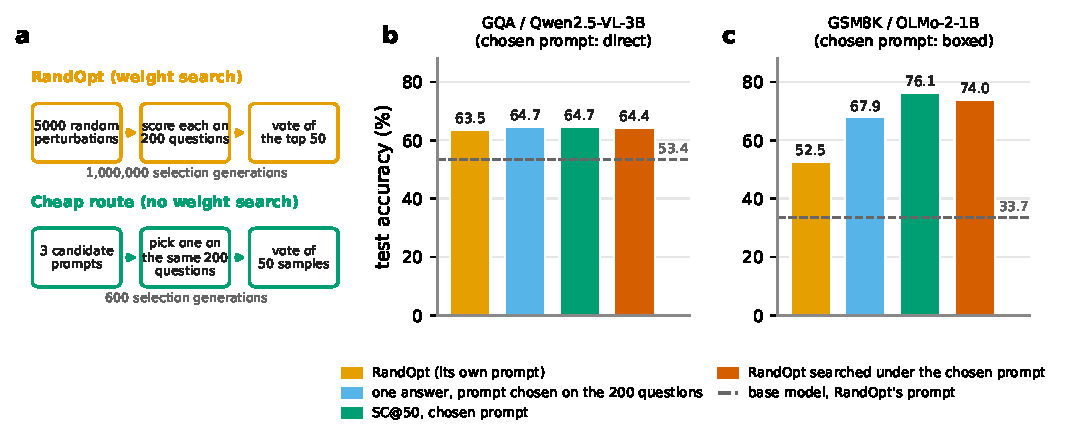
\includegraphics[width=\textwidth]{fig1_overview.pdf}
  \caption{\textbf{Choosing a prompt on RandOpt's own selection questions matches or beats its weight search, at 0.06\%
  of the selection compute.} (a) RandOpt scores 5000 random weight perturbations on 200 selection questions and votes the
  top 50; the cheap route picks one of three prompts on the same questions and votes 50 samples of the unperturbed
  model. (b, c) The two same-run rows where RandOpt beats self-consistency under its own prompt. RandOpt's prompt damages
  the base model (dashed); one answer under the chosen prompt already matches (GQA) or beats (OLMo) RandOpt, and
  re-running RandOpt's search under the chosen prompt adds nothing over sampling. GQA uses a faithful re-implementation
  of RandOpt.}
  \label{fig:overview}
\end{figure*}

% -----------------------------------------------------------------------------------------------------
\section{Background and Setup}\label{sec:setup}
\textbf{RandOpt.} Given a pretrained model with weights $\theta_0$, RandOpt \citep{gan2026thickets} draws $N$ seeds and
noise scales $\sigma \in \{0.0005, 0.001, 0.002\}$, forms $\theta_0 + \sigma\epsilon$ with $\epsilon$ a Gaussian vector
generated from the seed, scores each perturbed model by its reward on a selection set of 200 training questions under
greedy decoding, and answers each test question by a majority vote over the greedy answers of the top $K$. We use its
settings throughout: $N{=}5000$, $K{=}50$ ($K{=}10$ as a secondary), its prompts, answer extractors, scorers and vote
rule. This costs $5000 \times 200 = 1{,}000{,}000$ greedy generations for selection and 50 per test question.

\textbf{Rows.} GSM8K \citep{cobbe2021gsm8k} with Qwen2.5-1.5B-Instruct and Qwen2.5-3B-Instruct \citep{qwen2025qwen25}
(the original paper's models) and with OLMo-2-0425-1B-Instruct \citep{olmo2024olmo2} (a second family), evaluated on all
1319 test questions; and GQA \citep{hudson2019gqa} with Qwen2.5-VL-3B-Instruct \citep{bai2025qwen25vl}, evaluated on
1238 testdev questions whose images are disjoint from the selection questions' images. The GSM8K rows run RandOpt's
released script; its recomputed vote equals the count it prints. The released code cannot pass images to the model, so
the GQA rows use a re-implementation built on RandOpt's own perturbation, scoring and voting components. All model
revisions are pinned (Appendix~\ref{app:methods}).

\textbf{Baseline.} Self-consistency \citep{wang2023selfconsistency} (SC@$K$) majority-votes $K$ samples of the
\emph{unperturbed} model at temperature 0.7, with RandOpt's scorer and vote rule. SC@50 matches RandOpt's test-time
budget of 50 generations per question; RandOpt's selection generations are not charged to it.

\textbf{Statistics and protocol.} Every comparison is paired on the same test questions. We report differences $D$ in
accuracy points with 95\% confidence intervals from a paired item bootstrap (10{,}000 resamples); a method is
\emph{ahead} when the interval excludes zero, and two methods are \emph{equivalent} when it lies within $\pm 2$ points.
Confirmatory tests were specified in plan locks committed before their corresponding runs; exploratory analyses are
identified separately. Each lock fixes the comparison, its decision rule and its gates: a base-model reproduction or
environment check against an earlier independent measurement, a fidelity check against RandOpt's own logs where a
re-implementation is used, and a budget rule that stops a run rather than shrink it. Appendix~\ref{app:ledger} lists
every locked test with its outcome, including failed gates and runs that were not completed.

% -----------------------------------------------------------------------------------------------------
\section{What Weight Search Buys}\label{sec:buys}
% All numbers [R8b]; D = RandOpt - SC, paired 95% CI.
We run RandOpt at its own settings in four rows and compare it with self-consistency on the same test questions at
matched test-time budget (Table~\ref{tab:samerun}). We then ask what RandOpt's gain consists of, and whether something
cheaper than weight search supplies it.

\subsection{Same-run comparison under RandOpt's own prompts}\label{sec:samerun}
% [R8b.1]
RandOpt reproduces: on GSM8K its $K{=}50$ vote scores 77.18 with Qwen2.5-1.5B and 86.66 with Qwen2.5-3B, against the
published 76.4 and 87.1. Under RandOpt's own prompts, the comparison with \SC{} splits two ways. In the two Qwen GSM8K
rows self-consistency is ahead ($D = -2.65$ [$-4.32$, $-0.99$] and $-1.59$ [$-2.65$, $-0.53$]). On GQA RandOpt is ahead
($+3.47$ [$+1.62$, $+5.41$]), and a second search with a different population seed replicates this ($+3.63$ [$+1.78$,
$+5.49$]; seed-to-seed difference $+0.16$ [$-0.97$, $+1.29$]). On OLMo-2-1B, a model outside the original study,
RandOpt is ahead by $+8.72$ [$+6.75$, $+10.77$], and a second search with a different population, run with our
re-implementation, replicates this ($+10.39$ [$+8.26$, $+12.51$]). The published GQA number (69.0) uses all of testdev
with train-split selection and is not comparable to our image-disjoint split.

Under its own prompts, then, RandOpt is a real improvement over sampling in two of four rows. The rest of this section
asks what that improvement is.

\subsection{A vote and a shared shift}\label{sec:decomp}
% [R8b.1] members vs vote; vote efficiency and selection-set shares are EXPLORATORY.
RandOpt's gain can come from two places: each selected model may be better than the base model, or the vote over them
may correct errors that single models make. The mean single-model accuracy of the 50 selected models separates the two.
In the Qwen rows, where RandOpt loses, the selected models are only $+4.0$ (64.3 vs 60.3) and $+0.2$ (80.9 vs 80.7)
points above the base model individually: the gain is almost all vote, and sampling the unperturbed model votes better.
On GQA and OLMo, where RandOpt wins, the selected models are about 5 points above base individually (58.4 vs 53.4; 40.3
vs 35.25). That is a shift in answers shared across questions, which sampling cannot supply, since every sample comes
from the unchanged model.

Two exploratory measurements qualify this. Measured as the vote's gain over its own members' mean accuracy, sampling's
vote adds more than RandOpt's in three rows (Qwen-1.5B $+21.7$ vs $+12.9$; Qwen-3B $+9.9$ vs $+5.8$; GQA $+10.0$ vs
$+5.1$) and less on OLMo ($+10.1$ vs $+12.1$). And perturbations that beat the base model on the 200 selection questions
are common, 11.8--58.3\% of the 5000 depending on the row; the population mean is level with base on the Qwen rows
($-0.4$ and $-0.3$ points) and below it on GQA and OLMo.\footnote{For the Qwen rows we use the base selection accuracy
measured by the same engine that reproduces RandOpt's perturbed rewards (68.0 and 84.0). RandOpt's script prints 73.00
and 85.50 for the same 200 prompts, reproducibly across engine counts, while its test-set base agrees with ours (60.27
vs 60.05); we treat the print as engine-specific (Appendix~\ref{app:samerun}). No confirmatory comparison uses it.}

\subsection{The shift repairs damage done by RandOpt's own prompt}\label{sec:damage}
% [R8b.2 G3/G4 + exploratory shift analysis, R8b.3 O2, R8b.4 Q2, R8b.8 GQA agreement]
\textbf{GQA.} RandOpt's GQA prompt asks for step-by-step reasoning. Asking the base model for a direct answer instead
raises its greedy accuracy from 53.39 to 64.70 ($+11.31$ [$+8.48$, $+14.14$]). The selected perturbations largely stop
reasoning (exploratory): their median generation is 10 tokens against the base model's 146, 43.7\% of their outputs
contain step-by-step text against 97.0\%, and across the 50 members accuracy and mean length correlate at $r = -0.89$.
On the 616 test questions where the two base prompts disagree, the members give the direct prompt's answer 48.7\% of
the time and the step-by-step prompt's 15.3\%. Truncation explains only part of the gain: raising the token limit
from 256 to 1024 shrinks RandOpt's advantage by 0.97 [0.32, 1.70] points but leaves it at $+2.67$ [$+0.73$, $+4.52$].
A single direct-prompt generation of the base model scores 64.70, against RandOpt's 63.49 ($-1.21$ [$-2.83$,
$+0.40$], no difference detected).

\textbf{OLMo.} RandOpt's GSM8K instruction (``\ldots output the final answer after \#\#\#\#'') halves OLMo-2-1B's
accuracy: greedy 33.66, against 65.28 with the question alone and 67.85 with a boxed-answer instruction. Under the
plain prompt, \SC{} is ahead of RandOpt by 22.21 points ($-22.21$ [$-24.87$, $-19.56$]), and a single plain generation
by 12.81 [9.86, 15.69]. Unlike on GQA, the selected members do not answer like the better-prompted model
(exploratory): on the 878 questions where the boxed and RandOpt-prompt base answers disagree, they side with each about
equally often (24.1\% vs 27.7\%). Here the shift recovers accuracy without reproducing the better prompt's answers.

\textbf{Damage accompanies RandOpt's wins but does not decide them.} Our locked prediction was that RandOpt beats
\SC{} where its prompt damages the base model relative to a plain or direct prompt. It held in all four rows: the damage
was $+11.3$ (GQA) and $+31.6$ (OLMo) points where RandOpt won, and $+4.70$ [$+1.97$, $+7.43$] and $-7.20$ [$-9.55$,
$-4.78$] for Qwen-1.5B and Qwen-3B, where it lost. For the Qwen models the plain prompt is no fix: \SC{} under it
trails RandOpt ($+2.58$ [$+0.53$, $+4.62$] and $+7.05$ [$+5.23$, $+8.95$]). Measured post hoc against the prompt chosen
in Section~\ref{sec:ps}, Qwen-1.5B's damage is $+10.2$ and RandOpt still lost (Appendix~\ref{app:samerun},
Figure~\ref{fig:damage}), so damage alone does not decide the outcome.

\subsection{Choosing a prompt on RandOpt's own selection data}\label{sec:ps}
% [R8b.5] Headline. "matches or beats" (never "beats"). Robustness [R8b.6] in one sentence. RV-1, RV-5.
The controls above fix a prompt after seeing results. A practitioner can instead choose the prompt the way RandOpt
chooses perturbations: on its 200 selection questions. We fixed three candidates per task (GSM8K: RandOpt's prompt,
the question alone, a boxed-answer instruction; GQA: RandOpt's step-by-step prompt, a direct-answer prompt, a
short-answer prompt; Appendix~\ref{app:prompts}). Per row, we chose the candidate with the highest greedy base accuracy
on the selection questions and ran \SC{} under it on test. This costs 600 greedy generations against RandOpt's
1,000,000 (0.06\%). The rule chose the boxed prompt in all three GSM8K rows and the direct prompt on GQA.

Prompt selection followed by sampling matches or beats RandOpt in all four rows (Figure~\ref{fig:headline},
Table~\ref{tab:samerun}). It is ahead on Qwen-1.5B ($-2.96$ [$-4.62$, $-1.29$]) and OLMo ($-23.65$ [$-26.23$,
$-21.08$]). No difference is detected on Qwen-3B ($-0.38$ [$-1.67$, $+0.91$], equivalent within $\pm 2$ points) or on
GQA ($-1.21$ [$-2.83$, $+0.40$], not equivalent). The ordering holds under strict answer scoring and McNemar tests with
Holm correction, and with a $K{=}10$ vote, where RandOpt is ahead in no row (exploratory; Appendix~\ref{app:samerun}).
It does not depend on the sampling temperature: at $T = 0.5$ and $1.0$ the two no-difference rows stay no-difference
(pre-registered; Appendix~\ref{app:samerun}).

\textbf{Does the result depend on our candidates?} The three candidates were fixed before this test but chosen after
earlier results. We therefore repeated it with candidates we could not have tuned: public evaluation templates from
lm-evaluation-harness, simple-evals, LLaVA and BLIP-2, fixed in a plan lock before any of them was run, and chosen by
the same rule (Figure~\ref{fig:headline}, diamonds). Prompt-selected sampling then matches or beats RandOpt in three
rows: Qwen-3B ($-0.45$ [$-1.67$, $+0.76$], equivalent), OLMo ($-5.23$ [$-7.66$, $-2.81$]) and GQA ($-2.67$ [$-4.60$,
$-0.73$], now ahead). On Qwen-1.5B no public template beats RandOpt's own prompt on the selection questions (67.5 vs
68.5), and RandOpt is ahead ($+4.17$ [$+1.97$, $+6.44$]). Pooling all six candidates, the rule picks the boxed prompt
for the GSM8K rows and the LLaVA template for GQA, and matches or beats RandOpt in all four rows. The cheap route
therefore needs a candidate that fixes the answer format; a boxed-answer instruction, standard for math, is one.

\subsection{With the prompt held fixed, the search adds nothing}\label{sec:held}
% [R8b.2 GD, R8b.3 GB, R8b.9 RV-2a/RV-2b] Cite these only (not G4's re-used members; not O2 members: fidelity failed).
Prompt choice and weight search can be combined: RandOpt can be run under the chosen prompt. We re-ran its search, with
the same 5000 perturbations as in Section~\ref{sec:samerun}, under the direct prompt on GQA and the boxed prompt in the
three GSM8K rows (the latter with a fast re-implementation that passed its environment and fidelity gates). In every
row the top 50 again beat the base model on the selection questions (for example GQA 68.0--69.5\% vs 66.0\%; OLMo
84.0--86.0\% vs 79.5\%). On test, though, the selected models were no better than base in any row ($-0.60$ [$-1.27$,
$+0.05$] on GQA, $-0.81$ [$-2.19$, $+0.57$] on OLMo, $-0.47$ [$-1.45$, $+0.53$] on Qwen-3B, $-0.51$ [$-1.71$, $+0.73$]
on Qwen-1.5B), and RandOpt's vote never beat sampling (Table~\ref{tab:samerun}, Figure~\ref{fig:headline},
triangles). It was equivalent on GQA ($-0.32$ [$-1.29$, $+0.65$], within $\pm 2$ points) and behind on OLMo ($-2.12$
[$-3.49$, $-0.83$]), Qwen-3B ($-1.36$ [$-2.35$, $-0.38$]) and Qwen-1.5B ($-4.32$ [$-5.91$, $-2.81$]). On OLMo the
better prompt lifts RandOpt itself by 21.53 points [18.88, 24.18], yet it still trails sampling. The top 50 found
under the two prompts share no member in three rows and three members on Qwen-1.5B (Section~\ref{sec:selection}).

With the prompt held fixed, then, weight search added nothing measurable over sampling the unperturbed model in any of
the four rows. (The Qwen-1.5B search first failed a gate that compared our engine with the base accuracy printed by
RandOpt's script; we traced that print to an engine-specific effect, re-ran the search under gates that compare like
with like, and report the failed attempt in the ledger; Appendix~\ref{app:ledger}.)

\begin{figure}[t]
  \centering
  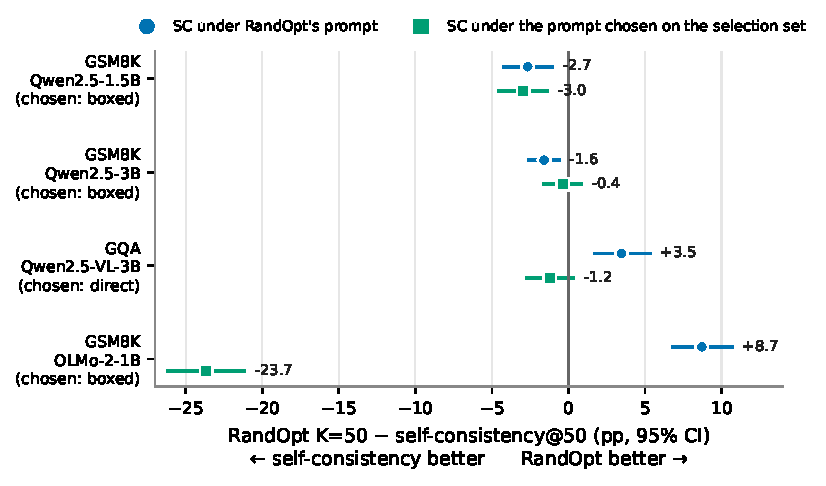
\includegraphics[width=\columnwidth]{fig7_same_run_prompt_selection.pdf}
  \caption{\textbf{Choosing a prompt on RandOpt's own selection data matches or beats its weight search in every row,
  and with that prompt held fixed the search adds nothing.} RandOpt ($K{=}50$) minus self-consistency ($K{=}50$) per
  row, paired 95\% CI: both under RandOpt's prompt (circles); SC under the prompt chosen on the 200 selection questions
  (squares) or under the public template chosen the same way (diamonds; on Qwen-1.5B no public template beats RandOpt's
  prompt and RandOpt is ahead); and RandOpt's search itself run under the chosen prompt (triangles). GQA uses a
  faithful re-implementation of RandOpt.}
  \label{fig:headline}
\end{figure}

\begin{table*}[t]
  \centering\small
  \caption{\textbf{Same-run results} ($N{=}5000$, $K{=}50$; accuracy in \%, differences in points with paired 95\% CIs).
  SC: self-consistency over 50 samples of the unperturbed model. The chosen prompt (in parentheses) maximizes base
  accuracy on RandOpt's 200 selection questions among our three candidates; the public template is chosen by the same
  rule among public evaluation templates fixed before any was run (Section~\ref{sec:ps}).}
  \label{tab:samerun}
  \footnotesize\setlength{\tabcolsep}{3pt}
  \resizebox{\textwidth}{!}{\begin{tabular}{lcccccc}
\toprule
 & \multicolumn{2}{c}{RandOpt's prompt} & \multicolumn{2}{c}{Prompt chosen on selection set} & \multicolumn{2}{c}{Search under chosen prompt} \\
\cmidrule(lr){2-3}\cmidrule(lr){4-5}\cmidrule(lr){6-7}
Row & RandOpt & RandOpt $-$ SC & SC@50 & RandOpt $-$ SC & RandOpt & RandOpt $-$ SC \\
\midrule
GSM8K / Qwen2.5-1.5B (boxed) & 77.2 & $-2.65$ {\scriptsize[$-4.32$, $-0.99$]} & 80.1 & $-2.96$ {\scriptsize[$-4.62$, $-1.29$]} & -- & -- \\
GSM8K / Qwen2.5-3B (boxed) & 86.7 & $-1.59$ {\scriptsize[$-2.65$, $-0.53$]} & 87.0 & $-0.38$ {\scriptsize[$-1.67$, $+0.91$]} & -- & -- \\
GQA / Qwen2.5-VL-3B (direct) & 63.5 & $+3.47$ {\scriptsize[$+1.62$, $+5.41$]} & 64.7 & $-1.21$ {\scriptsize[$-2.83$, $+0.40$]} & 64.4 & $-0.32$ {\scriptsize[$-1.29$, $+0.65$]} \\
GSM8K / OLMo-2-1B (boxed) & 52.5 & $+8.72$ {\scriptsize[$+6.75$, $+10.77$]} & 76.1 & $-23.65$ {\scriptsize[$-26.23$, $-21.08$]} & 74.0 & $-2.12$ {\scriptsize[$-3.49$, $-0.83$]} \\
\bottomrule
\end{tabular}
}
\end{table*}

% -----------------------------------------------------------------------------------------------------
\section{What a Perturbation Does to Answers}\label{sec:law}
% [R4, R5, R7]. Never "exact", never "noise alone".
Section~\ref{sec:buys} treated the selected perturbations as black boxes. Here we ask what a single perturbation does to
a model's answers, in the regime where that can be measured cleanly: direct answers, where each question has a
well-defined preference between candidate answers.

\textbf{A first-order prediction.} Let $c_j(\theta)$ be a contrast for question $j$, for example the log-probability of
one answer option minus another, or a tilt averaged over questions toward options containing a given content word. A
perturbation $\theta_0 + \sigma\epsilon$ changes it by
\begin{equation}
  \Delta c_j \approx \sigma \langle g_j, \epsilon \rangle, \qquad g_j = \mathrm{fold}\big(\nabla_\theta c_j(\theta_0)\big),
  \label{eq:law}
\end{equation}
where $\mathrm{fold}$ maps each parameter tensor's gradient onto the coordinates of RandOpt's shared noise stream
(Appendix~\ref{app:theory}). The prediction needs the base model's gradient and the perturbation's own noise; it has no
fitted coefficients. We reconstructed every perturbation byte-exactly from RandOpt's generator and verified it against
the engine's weights.

\textbf{It tracks the measurements across models and tasks} (Figure~\ref{fig:law}). For content tilts on two OmniSpatial
tasks, prediction and measurement correlate at $r = 0.938$ and $0.915$ (Qwen3-VL-8B), and at $0.925$ for Qwen2.5-VL-7B,
after a first attempt failed its reliability gate (0.52) and a remedy fixed in advance was applied (slopes 0.83--0.92
across these three tests). Per question, in RandOpt's own GQA setting with direct answers, $r = 0.930$ for $\sigma \le
0.002$. On a different family and a text-only task, OLMo-2-1B and OLMo-2-7B on ARC-Challenge \citep{clark2018arc}, $r =
0.790$ and $0.787$ (slopes 0.76 and 0.77). The law also holds item by item rather than only on average: the pooled
per-item correlation is $0.771$, with a per-item median of 0.88. In the first test, 99\% of the measured tilt variance
is answer content, not letter position. The prediction is first-order, not exact: slopes are below one and the scatter
is real.

\textbf{It is localized to the middle language layers} (Appendix~\ref{app:tilt}, Figure~\ref{fig:localization}).
Inserting the perturbation one block at a time, the block-level prediction holds at $r = 0.978$ (slope 0.95),
contributions add up ($r = 0.96$), and layers 6--23 of 36 carry 0.91 of the measured tilt variance (0.41, 0.22 and 0.28
for layers 6--11, 12--17 and 18--23; predicted 0.44, 0.22, 0.23). The middle layers carry most of the predicted
variance for a second task (0.73) and a second model (0.77).

\textbf{Its limits are as clear as its successes.} (i) \emph{Vision weights}: with the vision encoder perturbed too, the
whole-model first-order prediction of per-example contrasts fails its locked test ($r = 0.137$, falsified); the vision
group alone gives $r = 0.05$, while language groups give 0.71--0.96. (ii) \emph{Noise scale}: at $\sigma = 0.005$, beyond
RandOpt's grid, the law breaks in every model we tested ($r = 0.21$--$0.31$), consistent with second-order drift.
(iii) \emph{Chain of thought}: under RandOpt's step-by-step GQA prompt, 22\% of question--perturbation pairs flip
correctness at $\sigma \le 0.002$, unrelated to the first-order contrast (sign agreement 0.52). Perturbations and
sampling flip similarly susceptible questions (Spearman 0.946 between per-question flip propensities;
Appendix~\ref{app:tilt}), but perturbed models carry persistent effects across question sets ($r = 0.74$), so
perturbation is not pure re-sampling. The accounts of Sections~\ref{sec:law} and~\ref{sec:selection} therefore cover
the direct-answer regime; Section~\ref{sec:buys} rests on its own experiments.

\begin{figure*}[t]
  \centering
  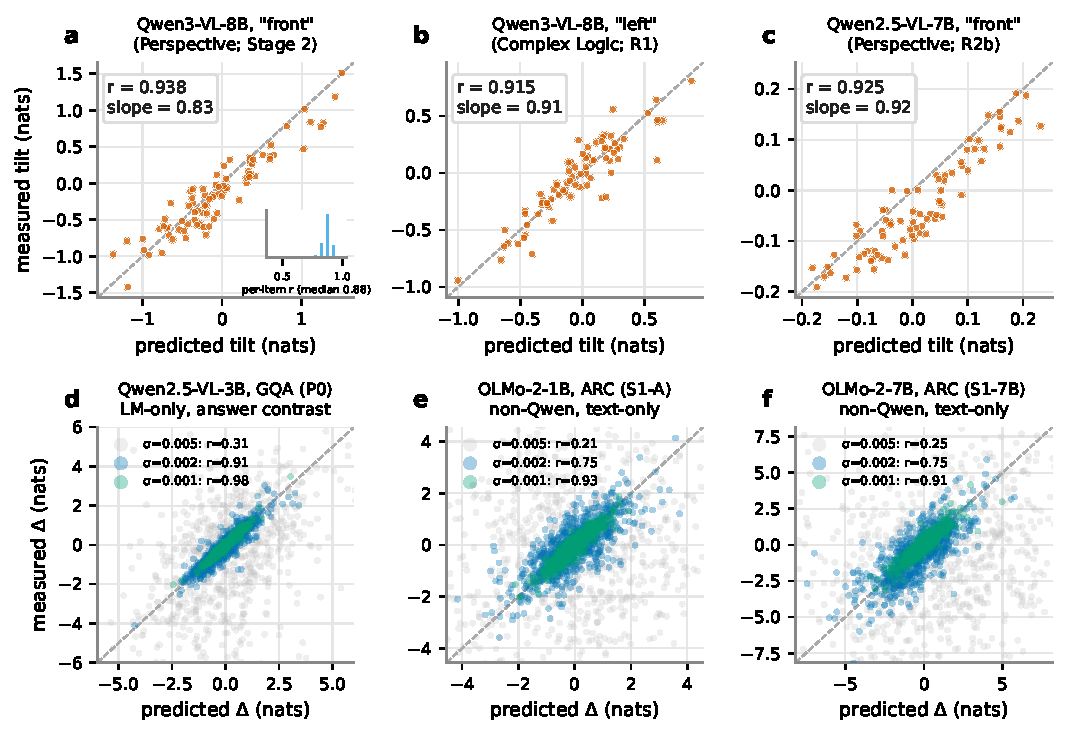
\includegraphics[width=\textwidth]{fig3_tilt_law.pdf}
  \caption{\textbf{A first-order prediction with no fitted coefficients tracks how perturbations shift answer
  preferences, across five models in two families.} (a--c) Answer-content tilts on two OmniSpatial tasks and two Qwen-VL
  models (slopes 0.83--0.92). (d--f) Per-question answer contrasts in RandOpt's GQA setting and on ARC-Challenge with the
  non-Qwen OLMo-2-1B and 7B, coloured by noise scale: the account holds at $\sigma \le 0.002$ and breaks at
  $\sigma{=}0.005$. Inset: per-item correlations (median 0.88).}
  \label{fig:law}
\end{figure*}

% -----------------------------------------------------------------------------------------------------
\section{Why Selection Finds Shared Shifts}\label{sec:selection}
% [R8b.7, R8b.8, R8c, R11, R1-R3]
\textbf{Selection gains transfer only where the prompt leaves accuracy unclaimed} (exploratory; Figure~\ref{fig:transfer}).
In every one of our ten $N{=}5000$ searches, the top 50 beat the base model on the 200 selection questions, while the
population mean is at or below base. Whether that gain survives on test depends on the prompt. Under a prompt that
damages the base model by 10 points or more, the selected models are better on test by 4.0--7.9 points (GQA and OLMo,
two searches each, and Qwen-1.5B); under RandOpt's prompt for Qwen-3B, which costs little, by 0.2; and under every
chosen prompt they are slightly worse than base ($-0.5$ to $-0.8$). In every search, selection found models that look
better on 200 questions; only a shared, prompt-repairing shift carried over.

\textbf{What selection finds is specific to the prompt} (exploratory; Figure~\ref{fig:experts}). Scoring the same 5000
perturbations under two prompts, their selection rewards are nearly unrelated (Spearman 0.025 on OLMo, 0.171 on GQA),
and the winners under RandOpt's prompt fall to the 37th and 31st percentile under the better prompt. On GQA the selected
perturbations reproduce the direct prompt's answers: where the two base prompts disagree, they side with the direct
one 48.7\% of the time against 15.3\%. On OLMo they do not (24.1\% vs 27.7\%). In our settings, then, the dense
``experts'' near the pretrained weights are repairs for a particular prompt rather than task experts.

\textbf{Why selection favours shared shifts.} Under Equation~\ref{eq:law}, a perturbation moves question $j$'s margin
by a Gaussian amount with standard deviation $\sigma\|g_j\|$ (Appendix~\ref{app:theory}). Three consequences follow,
which we checked against criteria fixed before computing them (exploratory, on existing data). A question flips with
probability $\Phi(-|c_j|/\sigma\|g_j\|)$, which predicts observed flips (AUC 0.935, calibrated within a factor of 1.41).
An unselected vote returns the base answer, as it does on 96 of 96 questions. And top-$K$ selection acts as a noisy
first-order step along the selection set's folded gradient: it rewards directions shared across the selection
questions, such as a format or answer-preference shift, and otherwise fits selection-set noise. This last step is
derived, not tested directly. The account covers direct answers at small $\sigma$; that the shared shifts we found are
ones a prompt also gives is an empirical finding of Section~\ref{sec:buys}, not a consequence of the theory.

\textbf{A case study at its boundary.} One OmniSpatial search (Qwen3-VL-8B, $N{=}5000$) produced a winner whose $+8.0$
point gain on its re-ranking set sat entirely on a question format (compass directions) that the official test set
nearly lacks (2 of 561 items); on fresh items matched to the selection data it keeps $+2.67$ [$+0.17$, $+4.93$]
(Appendix~\ref{app:omnispatial}). Selection had favoured a tilt toward the answer content the selection labels reward,
as the theory predicts. But removing that content shift leaves $+2.33$ of the $+2.67$ (not explained), and the full
first-order prediction does not explain which items the winner changes ($r = 0.16$, failing its locked test). The
winner's gain is also prompt-specific: under the benchmark's step-by-step prompts it becomes $-0.67$ [$-3.95$, $+2.51$]
or $-3.83$ [$-6.81$, $-0.84$], and a prompt chosen on the winner's own selection data gives the unperturbed model an
accuracy at least as high ($-1.50$ [$-5.35$, $+2.23$], no difference detected, not equivalent).

\begin{figure}[t]
  \centering
  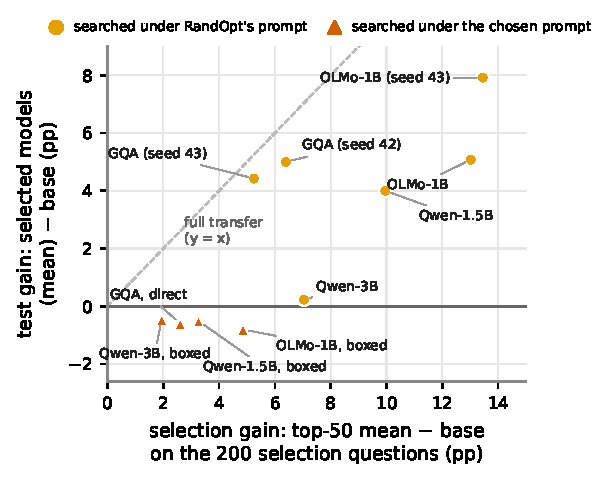
\includegraphics[width=\columnwidth]{fig10_transfer.pdf}
  \caption{\textbf{Selection gains transfer only where the prompt leaves accuracy unclaimed} (exploratory). Every
  search's top 50 beats the base model on the 200 selection questions; the selected models are better on test only
  under a damaging prompt, and in none of the four searches run under the chosen prompt (triangles).}
  \label{fig:transfer}
\end{figure}

\begin{figure}[t]
  \centering
  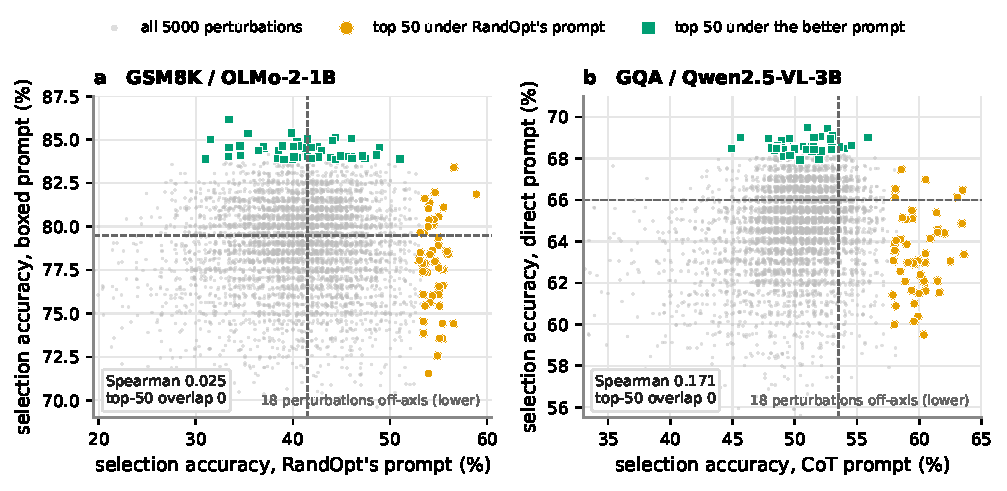
\includegraphics[width=\columnwidth]{fig9_prompt_specific_experts.pdf}
  \caption{\textbf{The selected ``experts'' are specific to the prompt} (exploratory). The same 5000 perturbations
  scored under two prompts: rank correlations 0.025 (OLMo) and 0.171 (GQA); the two top-50 sets share no member, and
  RandOpt's winners fall below the base model (dashed) once the prompt is improved.}
  \label{fig:experts}
\end{figure}

% -----------------------------------------------------------------------------------------------------
\section{Related Work}\label{sec:related}
\textbf{Random weight search.} RandOpt \citep{gan2026thickets} belongs to the family of zeroth-order, population-based
methods such as evolution strategies \citep{salimans2017evolution}, applied here as a single round of sampling and
selection around a pretrained model. Its authors already separate format from reasoning gains on GSM8K (``format
thickets''); our results agree with that reading and quantify it against cheap baselines. Concurrent work shows that
selection on small sets overfits in this setting and proposes Bayesian optimization over perturbations
\citep{bo2026thickets}; informal analyses discuss the geometry of the thicket \citep{blog_thicket_other_name} and when
RandOpt helps as a function of sequence length \citep{liu_when_randopt}. We add same-run baselines, controls that
isolate each component, and a tested account of what single perturbations do.

\textbf{Voting and prompts.} Self-consistency \citep{wang2023selfconsistency} is the natural baseline for any method
that votes over generations at test time; we find it supplies most of what RandOpt's vote supplies. Language models are
sensitive to prompt format \citep{sclar2024quantifying}; RandOpt's wins coincide with prompts that damage the base model,
and choosing among a few prompts on the selection data recovers them. Weight averaging \citep{wortsman2022soups}
combines models in weight space rather than voting over their outputs.

\textbf{Linear response.} Our first-order account is a linearization of the model around its pretrained weights in the
direction of each perturbation. Its use here is narrow: it predicts answer-preference shifts with no fitted
coefficients, and we report where it fails.

% -----------------------------------------------------------------------------------------------------
\section{Discussion, Recommendations and Limitations}\label{sec:discussion}
\textbf{What weight search buys, in our settings.} A vote, and shifts in answer form shared across questions. The vote
is available from sampling; the shifts were, in every row we tested, available from a prompt chosen on the same 200
selection questions, provided a format-fixing prompt is among the candidates. With that prompt held fixed, the search
added nothing in any row, and what selection found was specific to the prompt it ran under. This does not show that
nearby better models are absent: perturbations that beat the base model on the selection set are common (11.8--58.3\%),
and under a damaging prompt the selected ones are better on test. It shows that, at RandOpt's settings, what selection
recovers is what a prompt also recovers.

\textbf{Recommendations for evaluating weight-space search.} (1) Compare against self-consistency in the same run, at
the same test-time budget, with the same scorer. (2) Include a prompt chosen on the selection data as a baseline, with a
format-fixing candidate. (3) Report the selected models' individual accuracy next to the vote's, so the vote and the
shift can be told apart. (4) Report selection compute. (5) Check that the base model reproduces before comparing, and
compare like with like: in one case the same 200 prompts gave a base accuracy of 73.0\% in RandOpt's script and 68.0\%
in our engine, reproducibly.

\textbf{Limitations.} Two tasks and models up to 8B parameters; one RandOpt search per Qwen GSM8K row under its own
prompt (two on GQA and on OLMo), each row with a further search under the chosen prompt; RandOpt's selection set of 200
questions throughout, so we do not test whether larger selection sets change the picture; our prompt candidates were
chosen after earlier results, which the public-template test addresses for three of four rows; the first-order account
covers direct answers at small $\sigma$, not chain-of-thought correctness or vision weights, and does not explain most
of the OmniSpatial winner's gain. Exploratory analyses are labelled as such throughout.

% Required by ICML (check the current CFP for exact wording/placement):
\section*{Impact Statement}
This paper re-examines an evaluation and proposes cheaper baselines for it. It introduces no new capability. Its
main practical consequence is that a prompt chosen on a small selection set, followed by sampling, can replace a
weight search that costs more than 1,600 times as much selection compute, which reduces the compute spent on
post-training experiments of this kind.

\bibliography{refs}
\ifdefined\usingicml\bibliographystyle{\icmlstyle}\else\bibliographystyle{plainnat}\fi

% =====================================================================================================
\appendix
\onecolumn

\section{Confirmatory-Test Ledger}\label{app:ledger}
% R9, generated from RESULTS_MASTER by paper/figures/scripts/appendix_tables.py
Every locked test, with the rule fixed in its lock and its outcome, including falsified, inconclusive, gated-out and
skipped tests. A lock is the commit that fixed the rule before the output existed; amendments are recorded in the same
folders. Studies: GPU-A, Stage 1--3, R1, R2/R2b, I5, M1, C1, $\tau$-check, P0--P3, S1, S1-7B (the first-order account
and the OmniSpatial case study); C, C3B, G2, G2R, O1, PS, OS, GD, GB, Q2, O2, G4, G3, RV (Section~\ref{sec:buys}).
Engineering failures that produced no data (an offline-mode bug, a package conflict, a tar-ownership error, a budget rule
that skipped a RandOpt arm on a one-GPU pod) and the four pod interruptions during the RV runs are recorded in the
repository alongside the locks.
{\scriptsize\setlength{\tabcolsep}{3pt}\begin{longtable}{p{1.2cm}p{1.3cm}p{3.8cm}p{2.1cm}p{2.1cm}p{2.4cm}p{2.7cm}}
\toprule
Study & Lock & Test & Statistic & Rule (fixed in the lock) & Result & Outcome \\
\midrule
\endfirsthead
\toprule
Study & Lock & Test & Statistic & Rule & Result & Outcome \\
\midrule
\endhead
GPU-A run 1 & 198c352 & S2a HF vs vLLM fidelity & median per-item max \textbackslash{}|$\Delta$log p\textbackslash{}|; argmax agreement & $\le$ 0.10; $\ge$ 99\% & 0.25; 98\% & \textbf{NO-GO} (BF16 output resolution; led to amendment A1) \\
GPU-A A1 & 79252d4 & V0 score-definition gate; S2b candidate bytes & fp32 contrast checks; packed-tensor SHA & as locked & pass; 642/642 & pass \\
GPU-A A1 & 79252d4 & F1 whole-model first-order (vision perturbed) & pooled r, 13 candidates $\times$ 761 items & $\ge$ 0.6 support; $<$ 0.3 falsify & 0.137 & \textbf{falsified} \\
GPU-A A1 & 79252d4 & F2 changed answers predicted to flip & share & $<$ 0.5 falsify & 0.53 & not falsified (weak) \\
GPU-A A1 & 79252d4 & F3 RERANK gain prediction & r over 543 & $\ge$ 0.5 support; $<$ 0.3 falsify & 0.376 & inconclusive \\
GPU-A A1 & 79252d4 & S2d group partials vs insertions & pooled r & $<$ 0.5 falsify & 0.239 & \textbf{falsified} \\
Stage 1+2 & 09c1f1f & S1a reliability; S1b fidelity & Spearman--Brown; exactness & $\ge$ 0.7; all exact & 0.878; exact & pass \\
Stage 1+2 & 09c1f1f & \textbf{S2 tilt law} (Qwen3-VL-8B) & r(pred\_NOV, T\_NOV), 80 perturbations & $\ge$ 0.6 pass; $<$ 0.3 falsify & 0.938 (slope 0.83) & \textbf{pass} \\
Stage 1+2 & 09c1f1f & S2 share carried by non-vision & r(T\_NOV, T\_FULL)$^2$ & $\ge$ 0.5 & 0.843 & pass \\
Stage 3 & ce60c5d & 3A-0 pipeline consistency & r & $\ge$ 0.9 & 0.938 & pass \\
Stage 3 & ce60c5d & 3A-1 $\tau$ vs SEARCH gain & r over 5000 & $\ge$ 0.25 pass; $<$ 0.10 falsify & 0.240 & inconclusive \\
Stage 3 & ce60c5d & 3A-2 $\tau$ vs RERANK gain & r over 543 & same & 0.402 & pass \\
Stage 3 & ce60c5d & 3A-3 enrichment of advanced candidates & mean z difference & $\ge$ 0.3 SD & +0.09 [$-$0.01, 0.18] & not supported \\
Stage 3 & ce60c5d & 3B-1 block-level law & pooled r, 160 pairs & $\ge$ 0.6 pass; $<$ 0.3 falsify & 0.978 (slope 0.95) & \textbf{pass} \\
Stage 3 & ce60c5d & 3B-2 additivity; 3B-3 dominance & r; variance share & $\ge$ 0.9; $\ge$ 50\% for one block & 0.96; none & valid; distributed \\
R1 & 00155cc & reliability; position share; \textbf{law} & SB; share; r & $\ge$ 0.7; $<$ 0.20; $\ge$ 0.6 & 0.866; 0.184; \textbf{0.915} & \textbf{replicated} \\
R1 & 00155cc & middle-layer share & share of predicted variance, layers 6--23 & $\ge$ 0.5 & 0.73 & supported \\
R2 & 47d2102 & reliability; \textbf{law} (Qwen2.5-VL-7B, 96 items) & SB; r & $\ge$ 0.7; $\ge$ 0.6 & \textbf{0.518}; 0.920 & \textbf{inconclusive} (reliability gate failed) \\
R2b & 1cb3252 & reliability; position share; \textbf{law} (363 items; remedy fixed in advance) & SB; share; r & $\ge$ 0.7; $<$ 0.20; $\ge$ 0.6 & 0.949; 0.073; \textbf{0.925} & \textbf{replicated} \\
I5 & a1c2a7a & consistency gate; \textbf{per-item law} & r; pooled r, 7680 pairs & $\ge$ 0.99; $\ge$ 0.6 item-level, $<$ 0.3 average-only & 0.99999; \textbf{0.771} & \textbf{item-level} \\
M1 & 5eb864b & M1-1 winner on fresh matched items & gain, image-cluster CI & transfers if CI $>$ 0; full if also $\ge$ +6 & +2.67 [0.17, 4.93] & transfers (not full) \\
M1 & 5eb864b & M1-2 gold-front concentration & gain difference, CI & supports if CI $>$ 0 & +1.95 [$-$2.57, 6.47] & not supported \\
M1 & 5eb864b & M1-3 $\tau$ vs fresh gain & r over 59 (Fisher CI) & $\ge$ 0.25 supports & 0.61 [0.42, 0.75] & supports \\
M1 & 5eb864b & M1-4 top-50 vs controls & mean difference, bootstrap CI & reported & +1.16 [0.31, 2.03] & reported \\
C1 & 5aa4c06 & \textbf{C1-1 prior calibration of the winner} & calibrated vs raw fresh gain & explains if $\le$ 0.5$\times$raw with CI; not explained if $\ge$ 0.8$\times$raw & 2.33 vs 2.67 & \textbf{not explained} \\
C1 & 5aa4c06 & C1-2 surviving share (candidates with raw g $>$ 0) & $\Sigma$g\_cal / $\Sigma$g & $\le$ 0.5 supports & $\approx$ 0.00 [$-$0.42, 0.32] & locked label "supports"; \textbf{flagged}: a cross-fitted exploratory check shows it is regression-to-mean, so it is not evidence \\
$\tau$-check & 8c52ba1 & criteria fixed before computing (exploratory data) & within-top-50 r; partial r; control sign & $\ge$ 0.30; $\ge$ 0.20; $\ge$ 0 & 0.59; 0.31; 0.57 & holds (works through the front tilt) \\
P0 & d5152f7 & \textbf{per-question first-order} (LM-only GQA) & pooled r, $\sigma$ $\le$ 0.002 & $\ge$ 0.5 GO; $<$ 0.3 NO-GO & \textbf{0.930} & \textbf{GO} ($\sigma$ = 0.005: 0.31) \\
P1 & 464aed0 & P1-A flip propensities & Spearman over 400 items & $\ge$ 0.6 supports & 0.946 & supports \\
P1 & 464aed0 & P1-B persistence & r(selection, held-out) over 64 & persistent if $\ge$ 0.3 with CI $>$ 0 & 0.74 [0.61, 0.84] & \textbf{persistent} (rejects pure re-sampling) \\
P1 & 464aed0 & P1-C top-8 vote vs SC at T\textbackslash{}* & difference, item bootstrap CI & advantage if CI $>$ 0 & +2.5 [$-$3.5, 8.5] & no advantage (underpowered) \\
P2 & 01efd9d & base gate; SC@50 vs published RandOpt, GSM8K-1.5B & greedy diff; SC $-$ RandOpt & $\pm$2.0; match if $\ge$ $-$1.0 & 0.5; +3.4 & gate pass; MATCHES (label) \\
P2 & 01efd9d & same, GSM8K-0.5B / GQA-VL-3B & greedy diff & $\pm$2.0 / $\pm$2.5 & +3.3 / $-$2.6 & gate \textbf{fail}: not comparable \\
P3 & c60b600 & base gate; SC@50 vs published RandOpt, GSM8K-3B & greedy diff; SC $-$ RandOpt & $\pm$2.0; $\ge$ $-$1.0 & 0.5; +1.1 & gate pass; MATCHES (label) \\
P3 & c60b600 & same, MATH-500-1.5B / 3B & greedy diff & $\pm$2.0 & +6.4 / +5.8 & gate \textbf{fail}: not comparable \\
S1 & 797fa96 & \textbf{A-1 law on a non-Qwen model} (OLMo-2-1B, ARC-Challenge) & pooled r, $\sigma$ $\le$ 0.002, 1600 pairs & $\ge$ 0.5 GO; $<$ 0.3 NO-GO & \textbf{0.790} [0.753, 0.824] & \textbf{GO} \\
S1 & 797fa96 & B-1 winner per-item first-order (all parameters) & r over 600 fresh items & $\ge$ 0.5 GO; $<$ 0.3 NO-GO & 0.162 [0.067, 0.252] & \textbf{NO-GO} \\
S1 & 797fa96 & B-2 sign agreement on changed items & share, n = 52 & $\ge$ 0.70 supported; $<$ 0.60 not & 0.654 & inconclusive \\
C & 1437d44 + 6118222 & validity; base gate & recomputed = printed; $\pm$2.0 & exact; required & 1018 = 1018; +1.5 / +0.5 & valid; pass \\
C & 1437d44 + 6118222 & \textbf{C-1 same-run RandOpt (N = 5000, K = 50) $-$ SC@50} & paired item bootstrap & CI $>$ 0 RandOpt ahead; CI $<$ 0 SC ahead & \textbf{$-$2.65 [$-$4.32, $-$0.99]} & \textbf{SC AHEAD} \\
C & 1437d44 + 6118222 & K = 10 (secondary) & same & same & +1.97 [0.00, 3.87] & no difference detected \\
C3B & e78cfd0 & validity; base gate & recomputed = printed; $\pm$2.0 & required & 1143 = 1143; +0.9 / +0.5 & valid; pass \\
C3B & e78cfd0 & \textbf{C3B-1 same-run RandOpt $-$ SC@50, GSM8K-3B} & paired item bootstrap & as C-1 & \textbf{$-$1.59 [$-$2.65, $-$0.53]} & \textbf{SC AHEAD} \\
C3B & e78cfd0 & K = 10 & same & same & $-$1.06 [$-$2.35, 0.15] & no difference detected \\
G2 & d2b3d68 + 5be1720 & environment gate & base vs P2 greedy, same items & $\le$ 1.0 pp & 0.16 & valid \\
G2 & d2b3d68 + 5be1720 & \textbf{G2-1 same-run RandOpt $-$ SC@50, GQA} & paired item bootstrap & as C-1 & \textbf{+3.47 [+1.62, +5.41]} & \textbf{RANDOPT AHEAD} \\
G2 & d2b3d68 + 5be1720 & K = 10 & same & same & +4.36 [+2.26, +6.54] & RandOpt ahead \\
G2R & 9e84c4f + 0754376 & \textbf{G2R-1 GQA advantage with a disjoint population (seed 43)} & paired item bootstrap & REPLICATED if CI $>$ 0 & \textbf{+3.63 [+1.78, +5.49]}; D$_2$ $-$ D$_1$ +0.16 [$-$0.97, +1.29] & \textbf{REPLICATED} \\
O1 & e2e2400 & \textbf{O1-1 same-run RandOpt $-$ SC@50, GSM8K / OLMo-2-1B (non-Qwen)} & paired item bootstrap & as C-1 & \textbf{+8.72 [+6.75, +10.77]} & \textbf{RANDOPT AHEAD} (Claim 1 model-dependent on GSM8K) \\
O1 & e2e2400 & K = 10; O1b second seed & same; budget rule & -- & +7.58 [+5.31, +9.93]; O1b not run (\$87 $>$ \$58.5) & RandOpt ahead; skipped by rule \\
PS & a1caf88 & \textbf{PS: RandOpt K = 50 $-$ SC@50 under the prompt chosen on RandOpt's selection set} (Qwen-1.5B / Qwen-3B / OLMo / GQA) & paired item bootstrap & as G4 & \textbf{$-$2.96 [$-$4.62, $-$1.29] / $-$0.38 [$-$1.67, 0.91] / $-$23.65 [$-$26.23, $-$21.08] / $-$1.21 [$-$2.83, 0.40]} & \textbf{SC ahead / equivalent / SC ahead / n.d.: no row RandOpt ahead} \\
OS & c14ff18 & \textbf{OS-1 OmniSpatial winner (direct) $-$ BASE under the prompt chosen on SEARCH200 (manual\_cot)} & image-cluster bootstrap (as M1) & as G4 & \textbf{$-$1.50 [$-$5.35, +2.23]} & \textbf{NO DIFFERENCE DETECTED} (valid; answers identical to M1) \\
OS & c14ff18 & OS-2 winner gain with the prompt held fixed (manual\_cot) & same & reported & $-$0.67 [$-$3.95, +2.51] & no difference (under zeroshot\_cot $-$3.83 [$-$6.81, $-$0.84]) \\
GD & 0bb89eb & \textbf{GD-1 RandOpt searched under the direct prompt $-$ SC@50 direct, GQA (prompt held fixed)} & paired item bootstrap & as G4 & \textbf{$-$0.32 [$-$1.29, +0.65]} & \textbf{NO DIFFERENCE, EQUIVALENT ($\pm$2 pp)} (valid; finished on a second pod, cross-pod answers identical) \\
GB & 77332dd & \textbf{GB-1 RandOpt searched under the boxed prompt $-$ SC@50 boxed, GSM8K OLMo-2-1B (prompt held fixed)} & paired item bootstrap & as G4 & \textbf{$-$2.12 [$-$3.49, $-$0.83]} & \textbf{SC AHEAD} (env and fidelity gates passed) \\
GB & 77332dd & GB-2 same, Qwen2.5-1.5B & environment gate & $\pm$1.0 pp & base selection 68.00 vs 73.00 printed by randopt.py & \textbf{INVALID-ENV, not run} \\
Q2 & 2a55ccc & \textbf{Q2-1/2 RandOpt $-$ SC@50 with the plain prompt, Qwen 1.5B / 3B} & paired item bootstrap & as G4 & \textbf{+2.58 [0.53, 4.62] / +7.05 [5.23, 8.95]} & \textbf{RANDOPT AHEAD} (plain prompt is worse for Qwen) \\
Q2 & 2a55ccc & damage prediction (all four rows) & plain $-$ RandOpt-prompt base & supported if Qwen both $<$ 5 pp & +4.70, $-$7.20 (GQA +11.3, OLMo +31.6) & \textbf{supported} (4/4 rows, locked measure); not decisive: vs the PS-chosen prompt Qwen-1.5B damage is +10.2 and RandOpt still lost \\
O2 & 6ecafcf & \textbf{O2-1 RandOpt (O1) $-$ SC@50 with the plain question prompt, OLMo-2-1B} & paired item bootstrap & as G4 & \textbf{$-$22.21 [$-$24.87, $-$19.56]} & \textbf{PROMPT-SC AHEAD} (valid env) \\
O2 & 6ecafcf & member fidelity gate; search on top of prompt & answer agreement $\ge$ 0.90, acc $\le$ 2 pp & as locked & 0.70 / 0.63 pp; $-$0.91 [$-$2.27, 0.53] & \textbf{gate failed} $\rightarrow$ members secondary not valid \\
G4 & 2ad4e46 & \textbf{G4-1 RandOpt (CoT) $-$ SC@50 with a direct-answer prompt, GQA} & paired item bootstrap & as C-1, + equivalence $\pm$2 & \textbf{$-$1.21 [$-$2.83, +0.40]} & \textbf{NO DIFFERENCE DETECTED} (not equivalent) \\
G4 & 2ad4e46 & direct-prompt BASE $-$ CoT BASE; search on top of prompt & paired bootstrap & reported & +11.31 [8.48, 14.14]; $-$0.08 [$-$0.97, +0.81] & prompt effect; search adds nothing \\
G3 & dc19fd4 & \textbf{G3-1 does a 1024-token budget remove the GQA advantage?} & $\Delta$ = D256 $-$ D1024; D1024 & supported if $\Delta$ CI $>$ 0 and D1024 CI $\ni$ 0 & $\Delta$ +0.97 [0.32, 1.70]; D1024 +2.67 [0.73, 4.52] & \textbf{PARTIAL} \\
G3 & dc19fd4 & G3-2 base vs members non-termination at 256 & difference, CI & supported if CI $>$ 0 & +1.90 [0.31, 3.48] & supported (small) \\
S1-7B & d64a1ad & \textbf{7B-1 law at 7B} (OLMo-2-7B, ARC) & pooled r, $\sigma$ $\le$ 0.002 & $\ge$ 0.5 GO; $<$ 0.3 NO-GO & \textbf{0.787} [0.758, 0.820] & \textbf{GO} \\
RV & c33fec2 & \textbf{RV-1 RandOpt $-$ SC@50 under the public template chosen on the selection set} (Qwen-1.5B / Qwen-3B / OLMo / GQA) & paired item bootstrap & as PS & \textbf{+4.17 [+1.97, +6.44] / $-$0.45 [$-$1.67, +0.76] / $-$5.23 [$-$7.66, $-$2.81] / $-$2.67 [$-$4.60, $-$0.73]} & \textbf{RandOpt ahead / equivalent / SC ahead / SC ahead} (pooled six-candidate rule: SC ahead / equiv. / SC ahead / SC ahead) \\
RV & c33fec2 & \textbf{RV-2a RandOpt searched under boxed $-$ SC@50 boxed, Qwen2.5-3B (prompt held fixed)} & paired item bootstrap & as GB & \textbf{$-$1.36 [$-$2.35, $-$0.38]} & \textbf{SC AHEAD} (gates passed; resumed across sessions, amendment 1) \\
RV & c33fec2 & \textbf{RV-2b same, Qwen2.5-1.5B} (amendment 2; GB-2 re-run with the lock's gates) & paired item bootstrap & as GB & \textbf{$-$4.32 [$-$5.91, $-$2.81]} & \textbf{SC AHEAD} (gates passed) \\
RV & c33fec2 & \textbf{RV-3 second OLMo-2-1B search (seed 43), RandOpt $-$ SC@50 under RandOpt's prompt} (amendment 3) & paired item bootstrap & as O1 & \textbf{+10.39 [+8.26, +12.51]} & \textbf{RANDOPT AHEAD} (O1 replicated; gates passed) \\
RV & c33fec2 & RV-4 randopt.py base print, Qwen2.5-1.5B, fresh pod & reproduction & reading fixed in the lock & randopt.py 73.00 (4 and 1 engines) vs our runner 68.00 & \textbf{engine-specific base print}: fidelity limitation; exploratory R8b.1/R8b.7 recomputed \\
RV & c33fec2 & RV-5 SC@50 at T = 0.5 / 1.0 (Qwen-3B boxed; GQA direct) & paired item bootstrap & reported; T = 0.7 stays primary & $-$0.23 / $-$1.14; $-$1.05 / +0.24 (all CIs $\ni$ 0) & no outcome changes \\
\bottomrule
\end{longtable}
}

\section{Methods Details}\label{app:methods}
\textbf{Perturbations.} RandOpt generates one Gaussian stream per seed and assigns each parameter tensor a prefix of it;
$\mathrm{fold}$ in Equation~\ref{eq:law} maps per-tensor gradients onto that shared stream. Every perturbation used in
Sections~\ref{sec:law}--\ref{sec:selection} was reconstructed from RandOpt's generator and checked byte-exactly against
the serving engine's weights (packed-tensor hashes). For the same-run rows, our GQA re-implementation and the fast
GSM8K runner use RandOpt's \texttt{WorkerExtension} to apply and reset perturbations; the only stated deviation from
RandOpt's script is an exact reset from a stored base copy instead of subtract-to-restore. Fidelity gates compare the
rewards of the first 24 perturbations with those in RandOpt's own logs (mean absolute difference 0.0135--0.0181, no
systematic offset).

\textbf{Models and data.} Qwen2.5-1.5B-Instruct, Qwen2.5-3B-Instruct, Qwen2.5-VL-3B-Instruct, OLMo-2-0425-1B-Instruct,
OLMo-2-1124-7B-Instruct, Qwen2.5-VL-7B-Instruct and Qwen3-VL-8B-Instruct at pinned revisions; vLLM 0.11 in bfloat16;
greedy decoding (temperature 0, maximum 1024 tokens for GSM8K and 256 for GQA, as RandOpt) for selection and for the
selected models on test; self-consistency at temperature 0.7, top-$p$ 1, 50 samples with a fixed seed. GSM8K questions
and answers were checked identical across RandOpt's data files, the public dataset and every run (1319/1319). The GQA
selection set is RandOpt's 200 selection questions; the test set is a hash-selected sample of testdev with every
question whose image appears in the selection set removed (1238 questions).

\textbf{Decision rules.} Each lock states the primary comparison, the bootstrap, and the outcomes RANDOPT AHEAD, SC
AHEAD or NO DIFFERENCE DETECTED (plus EQUIVALENT when the interval lies within $\pm 2$ points), with gates on base
reproduction (within 1--2 points of an earlier independent measurement), environment and fidelity, and a budget rule
computed from a smoke run that stops a search rather than shrinks $N$.

\section{Additional Same-Run Results}\label{app:samerun}
\textbf{$K{=}10$.} Under RandOpt's prompts: Qwen-1.5B $+1.97$ [$0.00$, $+3.87$] (no difference), Qwen-3B $-1.06$
[$-2.35$, $+0.15$] (no difference), GQA $+4.36$ [$+2.26$, $+6.54$] and $+4.68$ [$+2.50$, $+6.95$] (second population),
OLMo $+7.58$ [$+5.31$, $+9.93$] and $+11.68$ [$+9.25$, $+14.10$] (second population). Against the prompt chosen on the
selection set: $-0.38$ [$-2.20$, $+1.52$], $-0.53$ [$-1.97$, $+0.91$], $-24.56$ [$-27.37$, $-21.83$], $-0.57$ [$-2.18$,
$+1.05$]; RandOpt is ahead in no row.

\textbf{Vote curves} ($K = 1/5/10/20/50$). Qwen-1.5B: RandOpt 68.2/74.6/77.2/77.5/77.2, SC 57.5/69.9/75.2/78.7/79.8.
OLMo (RandOpt's prompt): RandOpt 40.2/49.0/50.1/53.0/52.5.

\textbf{Robustness (exploratory).} With strict answer scoring (boxed-only or \#\#\#\#-only on GSM8K, exact match on
GQA) prompt-selected SC versus RandOpt on its own lenient scorer gives $-7.81$ [$-9.63$, $-6.06$], $-4.78$ [$-6.07$,
$-3.49$], $-26.00$ [$-28.58$, $-23.43$] and $-1.05$ [$-2.67$, $+0.57$]; the lenient scorer under-credits boxed answers
(Qwen-1.5B base 70.20 lenient vs 74.45 strict) and rescues RandOpt's prompt (60.05 vs 7.96 strict). McNemar tests with
Holm correction give $p = 0.0025$, 0.65, $\approx 4\times10^{-67}$ and 0.34 for the four rows; the GQA image-cluster
bootstrap gives [$-2.79$, $+0.41$].

\textbf{Temperature (RV-5, pre-registered).} SC@50 at $T = 0.5 / 0.7 / 1.0$ under the chosen prompt: Qwen-3B boxed
86.88 / 87.04 / 87.79, $D = -0.23$ [$-1.52$, $+1.06$] / $-0.38$ / $-1.14$ [$-2.50$, $+0.23$]; GQA direct 64.54 / 64.70 /
63.25, $D = -1.05$ [$-2.67$, $+0.65$] / $-1.21$ / $+0.24$ [$-1.53$, $+2.02$]. No outcome changes.

\textbf{Termination (G3).} Raising the GQA token budget from 256 to 1024 shrinks RandOpt's advantage by 0.97 [0.32,
1.70] but leaves $+2.67$ [$+0.73$, $+4.52$]; at 256 tokens the base model fails to terminate more often than the
selected models by 1.90 [0.31, 3.48] points. Termination explains about a quarter of the advantage.

\textbf{RandOpt's printed base accuracy (RV-4).} On a fresh pod, RandOpt's script prints a base selection reward of
73.00\% for Qwen2.5-1.5B with 4 engines and with 1 engine; our engine measures 68.00\% (and 68.5\% in an independent
earlier run) on the same 200 byte-identical prompts. The two engines agree on the perturbed rewards of the same 24
perturbations (signed mean difference $-0.001$) and on the test-set base (60.27 vs 60.05). For Qwen2.5-3B the print is
85.50 against our 84.00; for OLMo both give 41.50. We treat the print as an engine-specific effect of greedy
bfloat16 decoding on this model, use the same-engine base for the exploratory selection-set statistics of
Section~\ref{sec:decomp}, and note that a gate against this print caused our first Qwen-1.5B prompt-held-fixed search
to be declared invalid (ledger: GB-2); the search was re-run under gates that compare like with like (RV-2b).

\textbf{O2 member fidelity.} Rebuilding O1's selected models with exact weight reset reproduced their answers on only
70.2\% of items (accuracy within 0.63 points), most likely bfloat16 drift in RandOpt's subtract-to-restore; the
``search on top of the prompt'' secondary of that run is therefore not used, and Section~\ref{sec:held} rests on
searches run from scratch under the chosen prompt.

\begin{figure}[h]
  \centering
  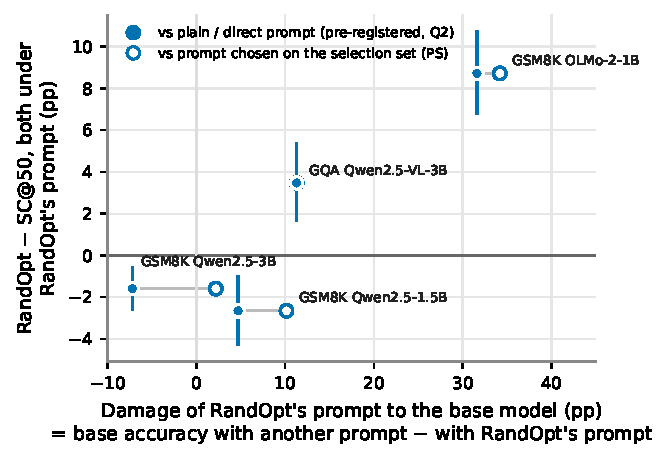
\includegraphics[width=0.6\textwidth]{fig8_prompt_damage.pdf}
  \caption{\textbf{Damage accompanies RandOpt's wins but does not decide them.} RandOpt minus SC@50 under RandOpt's
  prompt against the damage its prompt does to the base model, measured against a plain or direct prompt (filled,
  pre-registered) and against the prompt chosen on the selection set (open, post hoc). Qwen-1.5B is damaged by 10.2
  points on the post-hoc measure, and RandOpt still lost.}
  \label{fig:damage}
\end{figure}

\section{Theory Derivations}\label{app:theory}
% R11; checks R8c (criteria fixed before computing; exploratory)
\textbf{Setup.} $\theta' = \theta_0 + \sigma\epsilon$ with $\epsilon$ RandOpt's shared stream; for question $j$ the
answer margin is $c_j(\theta) = \mathrm{logit}(\text{gold}) - \mathrm{logit}(\text{strongest wrong answer at base})$.
The first-order law (Equation~\ref{eq:law}) gives $\Delta c_j \approx \sigma\langle g_j, \epsilon\rangle$.

\textbf{T1 (flip probability).} Since $\epsilon$ is isotropic Gaussian, $\langle g_j, \epsilon\rangle \sim
\mathcal{N}(0, \|g_j\|^2)$ over perturbations, so a random perturbation flips question $j$'s two-way answer with
probability $p_j(\sigma) = \Phi(-|c_j| / (\sigma\|g_j\|))$. Check (P0, Qwen2.5-VL-3B on GQA, $96 \times 16$ at $\sigma
\le 0.002$, $\|g_j\|$ estimated from predictions only): AUC 0.935 for the 46 observed flips; 65 predicted versus 46
observed (ratio 1.41, within the fixed range [0.67, 1.5]).

\textbf{T2 (unselected vote).} $\Delta c_j$ is symmetric about zero to first order, so each perturbation keeps the base
answer with probability $\Phi(|c_j|/(\sigma\|g_j\|)) > 1/2$ and the majority of $K$ unselected perturbations converges
to the base answer. Check: the majority over 16 perturbations equals the base answer on 96/96 questions. Beyond first
order, curvature adds a mean drift $\mathbb{E}[\Delta c_j] \approx \tfrac12\sigma^2\,\mathrm{tr}(\text{fold-Hessian})$;
at $\sigma = 0.005$ the mean margin drift is $-0.62$ [$-1.00$, $-0.27$], T1 loses discrimination (AUC 0.61) and the
vote departs from base on 2 of 96 questions, the same $\sigma$ at which the law breaks.

\textbf{T3 (selection as a first-order step).} Let the selection score be, to first order, $S(\epsilon) \approx S_0 +
\sigma\langle G_S, \epsilon\rangle$ with $G_S$ the folded gradient of a smoothed selection accuracy. Conditioning a
Gaussian $\epsilon$ on a high projection onto $u = G_S/\|G_S\|$ shifts only that component, $\mathbb{E}[\epsilon \mid
\text{selected}] = \mu_{K/N}\,u$ with $\mu_{K/N}$ the mean of the top-$K/N$ tail of $\mathcal{N}(0,1)$ ($\approx 2.67$
for the top 1\%), and leaves the orthogonal components as fresh noise. For any question $j$ a selected perturbation then
gives $\Delta c_j \approx \sigma\mu_{K/N}\|g_j\|\cos(g_j, G_S) + \mathcal{N}\big(0, \sigma^2\|g_j\|^2(1 - \cos^2(g_j,
G_S))\big)$. Gains transfer in proportion to a question's gradient alignment with the selection set, so shifts shared by
many items (a format or an answer-preference tilt) transfer and item-specific fits do not; the vote of selected models
keeps the common shift and, by T2, votes away the orthogonal noise. T3 is derived, not tested directly; the
noise-plus-gradient predictor correlates with re-ranking gains at $r = 0.40$ and with fresh-item gains at 0.61, working
through the content tilt.

\textbf{T4 (perturbations and sampling).} Temperature sampling flips question $j$ with probability $1/(1 +
\exp(|c_j|/T))$; a perturbation with $\Phi(-|c_j|/(\sigma\|g_j\|))$. Both decrease in the margin and differ only through
$\|g_j\|$, which varies moderately across questions (coefficient of variation 0.29), so $\sigma\|g_j\|$ acts as a
per-question effective temperature and the two mechanisms rank questions alike (model-implied Spearman 0.94). The
$\|g_j\|$ heterogeneity and the persistent common component of T3 are what distinguish perturbations from re-sampling.

\textbf{Not covered.} Chain-of-thought accuracy (multi-step generation compounds token-level shifts nonlinearly), vision
weights, $\sigma \ge 0.005$, and the OmniSpatial winner's residual gain.

\section{Tilt-Law Details}\label{app:tilt}
\begin{center}
\begin{tabular}{llllc}
\toprule
Test & Model & Contrast & $\sigma$ & $r$(predicted, measured) \\
\midrule
Stage 2 & Qwen3-VL-8B & front & 0.002 & 0.938 \\
R1 & Qwen3-VL-8B & left & 0.002 & 0.915 \\
R2b & Qwen2.5-VL-7B & front & 0.002 & 0.925 \\
I5 (per item, pooled) & Qwen3-VL-8B & front & 0.002 & 0.771 \\
P0 & Qwen2.5-VL-3B (LM-only) & per-question answer contrast & 0.001 & 0.977 \\
P0 & Qwen2.5-VL-3B (LM-only) & per-question answer contrast & 0.002 & 0.915 \\
P0 & Qwen2.5-VL-3B (LM-only) & per-question answer contrast & 0.005 & 0.306 \\
\bottomrule
\end{tabular}

\end{center}
Per noise scale, the per-question law gives $r = 0.977 / 0.915 / 0.306$ at $\sigma = 0.001 / 0.002 / 0.005$ for
Qwen2.5-VL-3B on GQA, $0.925 / 0.752 / 0.21$ for OLMo-2-1B and $0.914 / 0.755 / 0.25$ for OLMo-2-7B on ARC-Challenge.
Vision: with the vision encoder perturbed, the first-order standard deviation of the vision group's contribution is 7.1
nats against a measured 1.5, and adding the vision term lowers the full-perturbation fit from 0.84 to 0.53. For the
OmniSpatial winner evaluated per item on 600 fresh matched items with all parameters perturbed, the prediction gives
$r = 0.162$ [$0.067$, $0.252$] (failing its locked test); descriptively, the vision part carries 93\% of the
prediction's variance with $r = -0.008$, and the language part alone gives $r = 0.621$.

\begin{figure}[h]
  \centering
  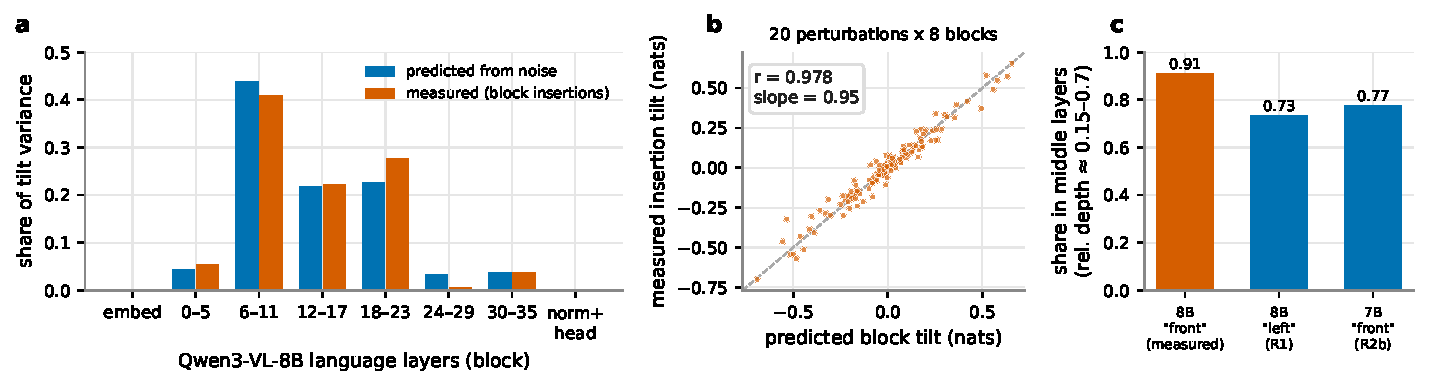
\includegraphics[width=0.6\textwidth]{fig4_localization.pdf}
  \caption{\textbf{The tilt lives in the middle language layers.} Share of the measured and predicted tilt variance by
  block for Qwen3-VL-8B (exact single-block insertions, 20 perturbations); the block-level prediction holds at $r =
  0.978$ and the contributions add ($r = 0.96$).}
  \label{fig:localization}
\end{figure}

\begin{figure}[h]
  \centering
  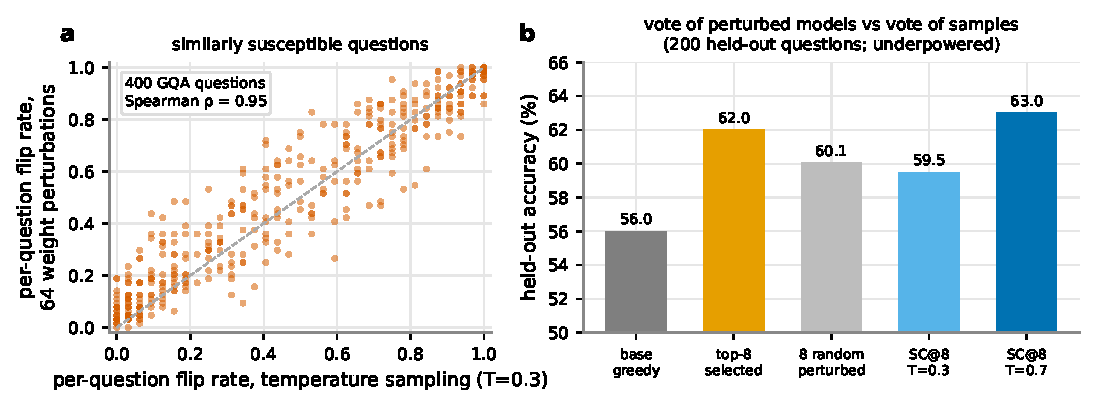
\includegraphics[width=0.8\textwidth]{fig6_cot_regime.pdf}
  \caption{\textbf{The chain-of-thought regime.} (a) Per-question flip rates under 64 weight perturbations and under
  temperature sampling of the base model are similarly ranked (Spearman 0.946) on 400 GQA questions: similarly
  susceptible questions, not an equivalent mechanism (perturbed models carry persistent effects, $r = 0.74$). (b) On 200
  held-out questions the vote of the top-8 selected perturbations (62.0) does not beat SC@8 (63.0 at $T = 0.7$; CI of the
  difference against SC at $T = 0.3$ [$-3.5$, $+8.5$], underpowered).}
  \label{fig:cot}
\end{figure}

\section{OmniSpatial Case Study}\label{app:omnispatial}
A pre-committed $N{=}5000$ search on Qwen3-VL-8B (all parameters including vision; $\sigma \in \{0.00025, 0.0005,
0.001, 0.002\}$) on OmniSpatial perspective taking \citep{omnispatial}, direct-letter prompt, in three stages: a
selection set of 200, a re-ranking set of 200 (543 candidates) and the official test set of 561 items. The winner
(seed 9504111, $\sigma = 0.002$) gained $+2.5$ points on selection and $+8.0$ on re-ranking, and lost $2.67$ on the
official test. The selection and re-ranking sets are 185/200 and 189/200 eight-way compass-format items; the official
test has 2 of 561 (Figure~\ref{fig:omni}a). The re-ranking gain lies entirely on compass items. On fresh items drawn
from the same source as the selection data (pre-registered, image-cluster bootstrap), the winner keeps $+2.67$
[$+0.17$, $+4.93$]; a gold-front concentration test is not supported ($+1.95$ [$-2.57$, $+6.47$]); the noise-plus-gradient
predictor correlates with fresh gain at $r = 0.61$ [$0.42$, $0.75$]; and the top 50 beat matched controls by $+1.16$
[$+0.31$, $+2.03$]. Removing the answer-content prior that selection favoured leaves $+2.33$ of the $+2.67$ (not
explained). A prompt control (pre-registered) shows the gain to be specific to the direct prompt: under the benchmark's
own step-by-step prompts the winner's gain is $-0.67$ [$-3.95$, $+2.51$] and $-3.83$ [$-6.81$, $-0.84$], and the
unperturbed model under the prompt chosen on the winner's selection data reaches 38.83 against the winner's 37.33
($-1.50$ [$-5.35$, $+2.23]$, no difference detected). Earlier conclusions drawn on the official test set before the
split mismatch was found are superseded and kept in the repository as a record.

\begin{figure}[h]
  \centering
  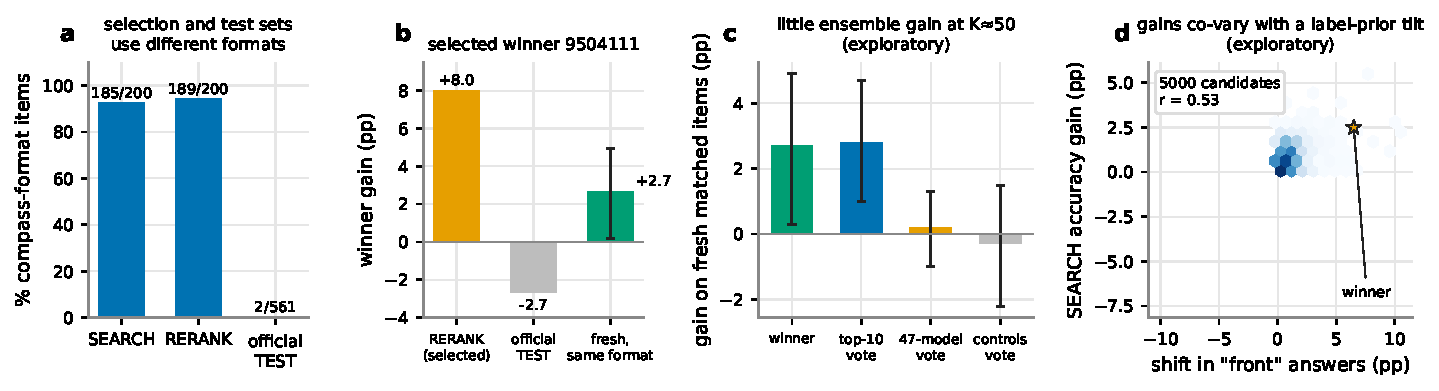
\includegraphics[width=\textwidth]{fig5_selection_transfer.pdf}
  \caption{\textbf{The OmniSpatial winner.} (a) Selection and test sets use different formats. (b) The winner's gain by
  stage; on fresh same-format items $+2.67$ [$+0.17$, $+4.93$]. (c) Little measured ensemble gain at $K \approx 50$
  (exploratory). (d) Across the 5000 candidates, selection gain co-varies with a tilt toward the answer content the
  selection labels reward ($r = 0.53$; exploratory).}
  \label{fig:omni}
\end{figure}

\section{Cross-Paper Comparisons}\label{app:crosspaper}
Before the same-run rows, we compared SC@50 of the unperturbed model with the RandOpt numbers published by
\citet{gan2026thickets}, gated on reproducing their base accuracy within 2 points. The gate passed for GSM8K with
Qwen2.5-1.5B and 3B, where SC@50 scores $+3.4$ and $+1.1$ points above the published RandOpt and 5.7--10.7 points above
the published test-time majority-vote baseline; it failed for GSM8K-0.5B, GQA and MATH-500, which are therefore not
comparable. These comparisons are across papers and are superseded by Section~\ref{sec:buys}.
\begin{center}\small
\begin{tabular}{llcccccc}
\toprule
Task & Model & Base (ours / paper) & Gate & SC@50 & TT-MV$^\dagger$ & RandOpt$^\dagger$ & Verdict \\
\midrule
GSM8K & Qwen2.5-1.5B & 59.3 / 58.8 & pass & 79.8 [77.6, 82.0] & 69.1 & 76.4 & matches \\
GSM8K & Qwen2.5-3B & 80.3 / 79.8 & pass & 88.2 [86.5, 90.1] & 82.5 & 87.1 & matches \\
GSM8K & Qwen2.5-0.5B & 43.2 / 39.9 & fail & 56.0 [53.1, 58.6] & 41.0 & 54.1 & not comparable \\
MATH-500 & Qwen2.5-1.5B & 49.6 / 43.2 & fail & 62.4 [58.2, 66.6] & 50.0 & 59.7 & not comparable \\
MATH-500 & Qwen2.5-3B & 64.4 / 58.6 & fail & 73.8 [70.0, 77.6] & 60.8 & 68.7 & not comparable \\
GQA (2000) & Qwen2.5-VL-3B & 54.0 / 56.6 & fail & 59.2 [57.1, 61.4] & -- & 69.0 & not comparable \\
\bottomrule
\end{tabular}

\end{center}
\begin{figure}[h]
  \centering
  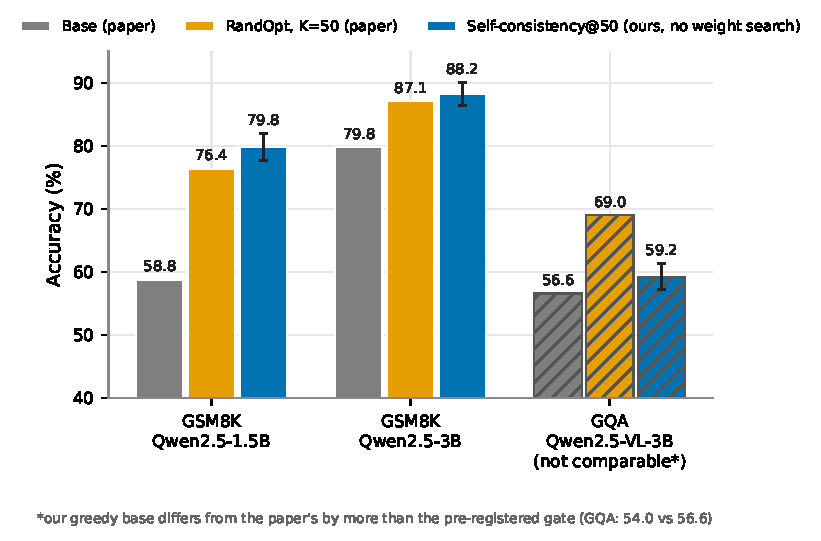
\includegraphics[width=0.48\textwidth]{fig1b_sc_vs_randopt.pdf}\hfill
  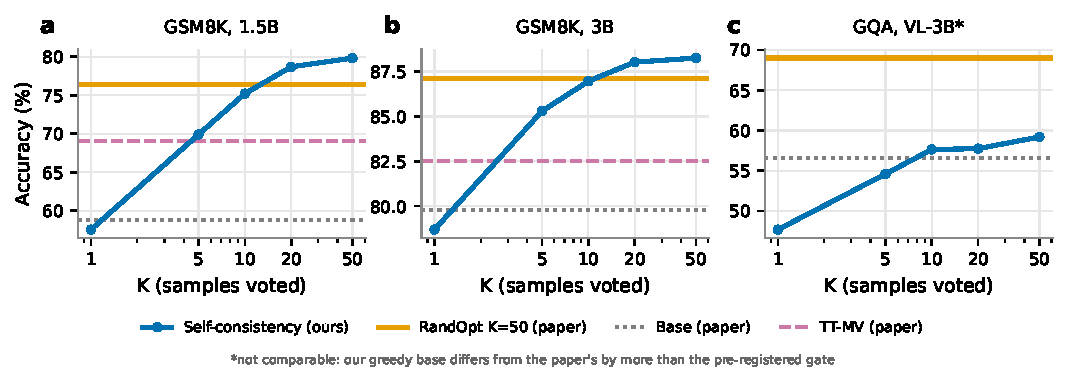
\includegraphics[width=0.48\textwidth]{fig2_sc_at_k.pdf}
  \caption{\textbf{Cross-paper comparison} (published RandOpt numbers, not same-run). Left: SC@50 versus the published
  RandOpt and majority-vote numbers on the gated rows. Right: SC@$K$ as a function of $K$.}
\end{figure}

\section{Prompts and Scorers}\label{app:prompts}
All prompts are applied through each model's chat template as a single user message; RandOpt's scorers extract the
answer (GSM8K: the number after \#\#\#\#, else the last number in the response; GQA: the \texttt{boxed} content, else
a short final answer or first line) and compare it with the reference. The candidates of Section~\ref{sec:ps}, verbatim
(\texttt{\{q\}} is the question):
\begin{itemize}\small
  \item GSM8K, RandOpt's prompt: \texttt{\{q\} Let's think step by step and output the final answer after "\#\#\#\#".}
  \item GSM8K, plain: \texttt{\{q\}}
  \item GSM8K, boxed: \texttt{\{q\}\textbackslash nPlease reason step by step, and put your final answer within \textbackslash boxed\{\}.}
  \item GQA, RandOpt's prompt (step by step): \texttt{Look at the image and answer the question.} [two line breaks] \texttt{Question: \{q\}} [two line breaks] \texttt{Please reason step by step, and put your final answer within \textbackslash boxed\{\}.}
  \item GQA, direct: the same with \texttt{Answer directly without explanation, and put your final answer within \textbackslash boxed\{\}.}
  \item GQA, short: the same with \texttt{Answer the question using a single word or phrase, and put your final answer within \textbackslash boxed\{\}.}
\end{itemize}
The public templates (fixed in the RV lock before any was run): lm-evaluation-harness \texttt{gsm8k\_cot\_zeroshot}
(\texttt{Q: \{q\}\textbackslash nA: Let's think step by step.}), lm-evaluation-harness \texttt{gsm8k} (\texttt{Question:
\{q\}\textbackslash nAnswer:}), the openai/simple-evals math template (\texttt{Solve the following math problem step by
step. The last line of your response should be of the form Answer: \$ANSWER (without quotes) where \$ANSWER is the
answer to the problem.\textbackslash n\textbackslash n\{q\}\textbackslash n\textbackslash nRemember to put your answer on
its own line after "Answer:".}), the LLaVA-1.5 GQA template (\texttt{\{q\}\textbackslash nAnswer the question using a
single word or phrase.}) and the BLIP-2 template (\texttt{Question: \{q\} Short answer:}). Their base accuracies on the
200 selection questions were 60.0 / 65.0 / 67.5 (Qwen-1.5B), 77.5 / 72.0 / 89.0 (Qwen-3B), 8.0 / 31.0 / 58.0 (OLMo) and
67.0 / 64.0 (GQA, LLaVA / BLIP-2).

\section{Compute}\label{app:compute}
All runs used rented H100 80GB pods (vLLM 0.11). Recorded costs per study: same-run RandOpt searches with RandOpt's
script, \$46 (Qwen-1.5B), \$52 (Qwen-3B) and \$47 (OLMo); GQA searches \$23 and \$31 (second population); the
prompt-held-fixed searches \$21 (GQA) and \$19 (OLMo); the reviewer round \$87 (public templates, two Qwen
prompt-held-fixed searches, a second OLMo population, the engine diagnosis and the temperature check); the prompt
controls and prompt selection \$3--6 each; the first-order-law measurements \$1--5 each; the OmniSpatial transfer and
prompt controls \$6 and \$2. The studies reported here sum to roughly \$400 of GPU time, excluding the original
OmniSpatial search.

\end{document}
